\chapter{Related Work}
Um diese Arbeit in einen wissenschaftlichen Kontext zu setzen, wird im Folgenden ein Überblick über aktuelle Arbeiten aus dem Feld SmartNIC und BlueField gegeben.
\begin{figure}
    \centering
    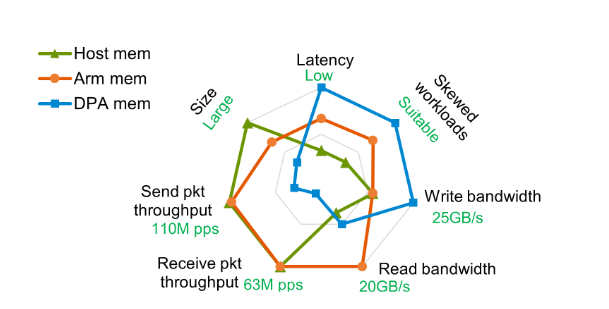
\includegraphics[width=0.7\linewidth]{images/DPARam.png}
    \caption{Vergleich der Speicher der Architekturen \cite{chen2024demystifying}}
    \label{fig:enter-label}
\end{figure}
\section{Demystifying Datapath Accelerator Enhanced Off-path SmartNIC}
\textit{Diese Arbeit wurde von Xuzheng Chen, Jie Zhang, Ting Fu, Yifan Shen, Shu Ma, Kun Qian, Lingjun Zhu, Chao Shi, Yin Zhang, Ming Liu und Zeke Wang verfasst. Sie ist an der Zhejiang University, Alibaba Cloud und der University of Wisconsin–Madison entstanden.}

In diesem Paper wird ein allgemeiner Performance-Kontext erstellt. Dabei liegt der besondere Fokus auf der Analyse und der Leistung des Datapath Accelerators (DPA). Dieser ist auf allen Generationen BlueField verbaut worden, wird allerdings kaum in dem Material von NVidia erwähnt. Allerdings handelt es sich beim DPA um die relevanteste Hardwareeinheit für die Netzwerkfunktionalität. 

In der Arbeit wird auch ein Vergleich zwischen dem Host-System, dem ARM-System und dem DPA selbst gezogen. Dabei werden die Metriken Latenz, verzerrte Lasten, Schreib- und Lesebandbreite, Sende- und Empfangspaketbandbreite u. a. ausgewertet (siehe Abbildung 3.1). Die Autoren identifizieren den verbauten DPA als einen RV64IMAC. Dies ist ein RISC-V-Prozessor mit einem Basistakt von 1.8 GHz. Sie entwickeln drei unterschiedliche Benchmark-Methoden, um eine Baseline zu schaffen, die alle drei verfügbaren Architekturen sinnvoll miteinander vergleicht. Die Autoren erkennen den DPA als einen der eventuellen Schwachpunkte einer spezifischen Implementierung. Die besondere Kritik liegt dabei auf der fehlenden Dokumentation seitens NVidia, die es so den Entwickelnden der Plattform deutlich erschwert, Software für diese zu entwickeln.

\section{Performance Characteristics of the BlueField-2 SmartNIC}
\textit{Diese Arbeit wurde von Jianshen Liu, Carlos Maltzahn, Craig Ulmer und Matthew Leon Curry verfasst. Sie ist an der UC Santa Cruz und den Sandia National Laboratories entstanden.}

Abermals geht es in dieser Arbeit um die allgemeine Performance der BlueField-2. Allerdings wird hier neben der gegebenen Hardware auch die Netzwerkfähigkeit überprüft. Die ARM-Kerne werden mittels Netzwerkaufgaben stark belastet, um die oberen Grenzen für Abhängigkeiten im Datenfluss zu erkennen. Das Paper ist von besonderem Interesse im Kontext dieser Bachelorarbeit, da die echte Leistung der BlueField-2-Generation mit der beworbenen Netzwerkbandbreite verglichen wird. Die Autoren implementieren einen Testfall, bei dem Netzwerkverkehr zwischen dem Host, der Smart NIC und einem weiteren Remote-Host stattfindet. Sie kommen zu dem Ergebnis, dass nur sehr schwer und unter einer Menge von Umständen überhaupt die volle Netzwerkbandbreite verwendet werden kann. Hauptsächlich ist die Leistung von der spezifischen Arbeitslast abhängig. Somit sollte vor einer Implementierung abgewogen werden, um festzustellen, ob sich das Offloading überhaupt auf eine Smart NIC-Architektur lohnt.
\section{A Comprehensive Survey on SmartNICs: Architectures, Development Models, Applications, and Research Directions}
\textit{Diese Arbeit wurde von Elie Kfoury, Samia Choueiri, Ali Mazloum, Ali AlSabeh, Jose Gomez und Jorge Crichigno verfasst. Sie ist an der University of South Carolina entstanden.}

Dieses Paper stellt einen guten Überblick über Smart NICs im Allgemeinen dar. Außerdem wird die Entwicklung der Architekturen der SmartNICs historisch aufgearbeitet. Es kann als eine Art Metapaper betrachtet werden, da auch ein Ausblick gegeben wird, was in Zukunft auf den jeweiligen Plattformen von Interesse sein könnte. Es wird ein klarer Zusammenhang zwischen dem Ende des Mooreschen Gesetzes und der fehlenden weiteren Leistungssteigerungen bei normalen Prozessoren mit dem Aufkommen von Smart NICs hergestellt. Es wird zwischen den drei folgenden Typen von Netzwerkkarten unterschieden:
\begin{itemize}
    \item Network Interface Cards beschreiben klassische Netzwerkkarten ohne weitere programmierbare Funktionalität.
    \item Offload-NICs bieten eine Einbettung von einigen Hardwarebeschleunigern für bestimmte Aufgabenbereiche.
    \item Smart-NICs beschreiben die Kombination aus klassischen Prozessoren mit anwendungsbezogenen speziellen Prozessoren und Hardwarebeschleunigern.
\end{itemize}
Innerhalb der Klasse von Smart-NICs treffen die Autoren außerdem die weitere Unterscheidung zwischen FPGA- und ASIC-basierten Smart NICs. Es wird angeraten, eine standardisierte Programmierungsplattform zu entwickeln, die es erlaubt, für alle Smart NIC-Plattformen zu programmieren.
\section{Laconic: Streamlined Load Balancers for SmartNICs}
\textit{Diese Arbeit wurde von Tianyi Cui, Chenxingyu Zhao, Wei Zhang und Kaiyuan Zhang  verfasst. Sie ist an der University of Washington und bei Microsoft entstanden.}
\begin{figure}
    \centering
    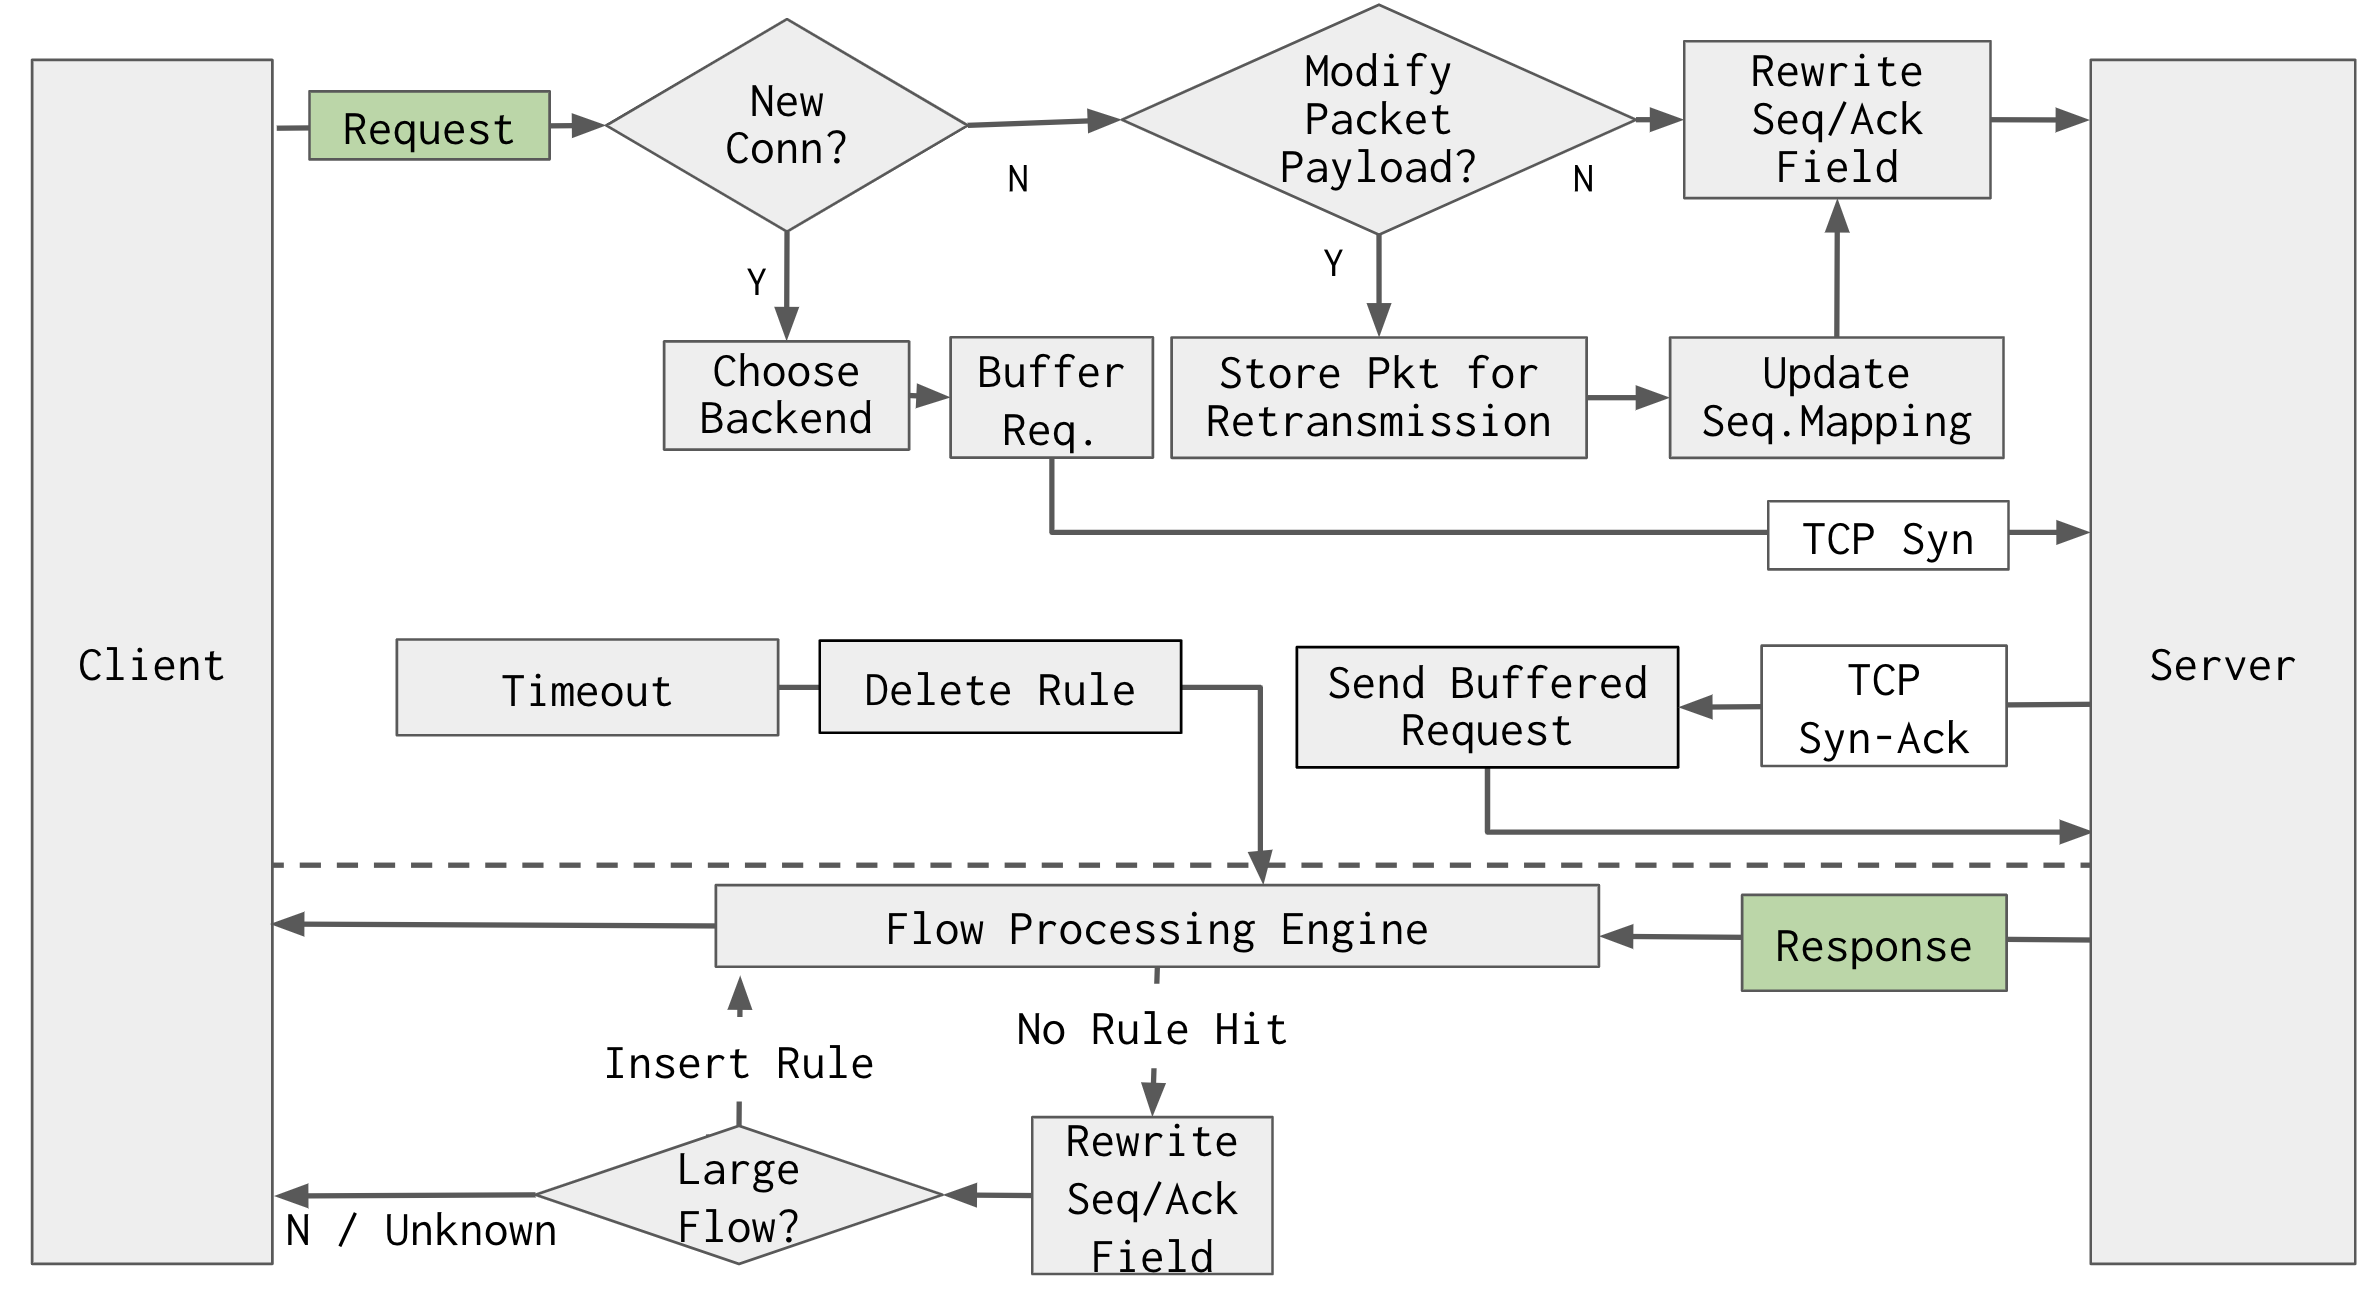
\includegraphics[width=1\linewidth]{images/laconic_workflow_v1.png}
    \caption{Leichtgewichtiger Netzwerkstack des Laconic LB}
    \label{fig:enter-label}
\end{figure}

Dieses Paper kommt dieser Arbeit auf fachlicher Ebene wohl am nächsten und wäre von Seiten des Quelltextes eine gute Referenz gewesen. Leider wurde der besagte Quelltext allerdings nicht veröffentlicht, und es konnte somit kein Bezug auf diese Arbeit genommen werden.
In ihrer Arbeit beschreiben die Autoren, wie wichtig L7-Lastverteilung für moderne Workloads geworden ist. Dazu stellen sie einen Bezug zu den Energiekosten von aktuellen L7-Lastverteilern her, wobei natürlich die hohen Energiekosten im Mittelpunkt stehen. Die meisten Optimierungen mittels Hardwarebeschleuniger wurden laut den Autoren vor allem auf L4 des OSI-Modells durchgeführt. Deshalb ist ihr Ansatz, auf einer Smart-NIC-Architektur einen besagten Lastverteiler zu implementieren. Als Referenz wählen sie dazu den Nginx als Softwarelastverteiler. Der Lastverteiler wird von den Autoren Laconic genannt. Dieser beinhaltet auch einen komplett eigenen Netzwerkstack auf der BlueField, der so laut den Autoren komplett ohne TCP/IP-Stack arbeiten kann (siehe Abbildung 3.2). Besagter Stack erlaubt es ihnen, sehr schnell und vor allem hardwarebeschleunigt auf der Smart NIC zu verteilen. Dazu setzen sie stark auf gute Parallelität der Algorithmen, um möglichst effizient die zur Verfügung stehenden 256 Threads des DPA zu verwenden. Sie zeigten also erstmalig, dass ein leichterer Stack, der speziell für die entsprechende Hardware entwickelt wurde, wesentlich schneller sein kann als eine vergleichbare Anwendung auf einem x86-Prozessorkern. Sie erreichen einen Speedup von 8.7 gegenüber dem klassischen Nginx.